% Created by tikzDevice version 0.12.3.1 on 2021-12-16 01:48:07
% !TEX encoding = UTF-8 Unicode
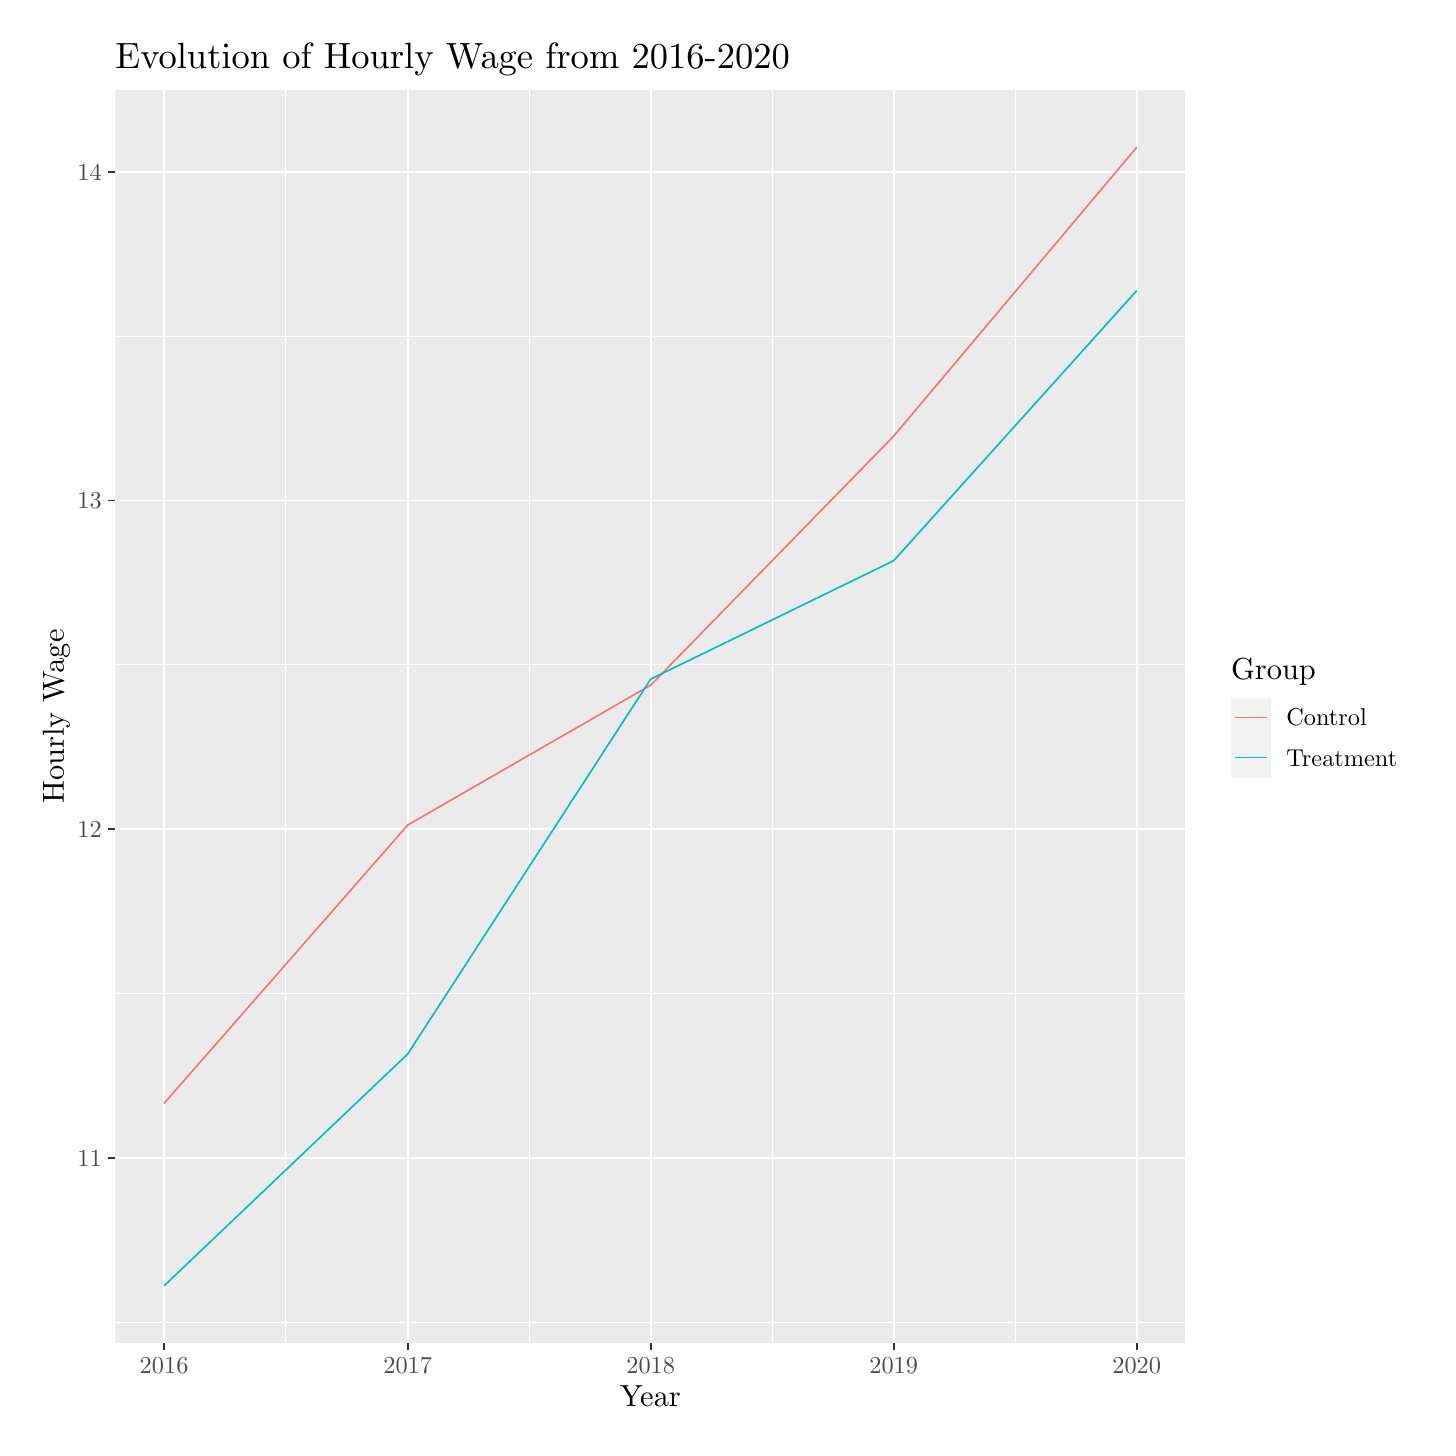
\begin{tikzpicture}[x=1pt,y=1pt]
\definecolor{fillColor}{RGB}{255,255,255}
\path[use as bounding box,fill=fillColor,fill opacity=0.00] (0,0) rectangle (505.89,505.89);
\begin{scope}
\path[clip] (  0.00,  0.00) rectangle (505.89,505.89);
\definecolor{drawColor}{RGB}{255,255,255}
\definecolor{fillColor}{RGB}{255,255,255}

\path[draw=drawColor,line width= 0.6pt,line join=round,line cap=round,fill=fillColor] (  0.00,  0.00) rectangle (505.89,505.89);
\end{scope}
\begin{scope}
\path[clip] ( 31.71, 30.69) rectangle (418.33,483.23);
\definecolor{fillColor}{gray}{0.92}

\path[fill=fillColor] ( 31.71, 30.69) rectangle (418.33,483.23);
\definecolor{drawColor}{RGB}{255,255,255}

\path[draw=drawColor,line width= 0.3pt,line join=round] ( 31.71, 38.12) --
	(418.33, 38.12);

\path[draw=drawColor,line width= 0.3pt,line join=round] ( 31.71,156.89) --
	(418.33,156.89);

\path[draw=drawColor,line width= 0.3pt,line join=round] ( 31.71,275.67) --
	(418.33,275.67);

\path[draw=drawColor,line width= 0.3pt,line join=round] ( 31.71,394.44) --
	(418.33,394.44);

\path[draw=drawColor,line width= 0.3pt,line join=round] ( 93.31, 30.69) --
	( 93.31,483.23);

\path[draw=drawColor,line width= 0.3pt,line join=round] (181.24, 30.69) --
	(181.24,483.23);

\path[draw=drawColor,line width= 0.3pt,line join=round] (269.05, 30.69) --
	(269.05,483.23);

\path[draw=drawColor,line width= 0.3pt,line join=round] (356.85, 30.69) --
	(356.85,483.23);

\path[draw=drawColor,line width= 0.6pt,line join=round] ( 31.71, 97.51) --
	(418.33, 97.51);

\path[draw=drawColor,line width= 0.6pt,line join=round] ( 31.71,216.28) --
	(418.33,216.28);

\path[draw=drawColor,line width= 0.6pt,line join=round] ( 31.71,335.06) --
	(418.33,335.06);

\path[draw=drawColor,line width= 0.6pt,line join=round] ( 31.71,453.83) --
	(418.33,453.83);

\path[draw=drawColor,line width= 0.6pt,line join=round] ( 49.29, 30.69) --
	( 49.29,483.23);

\path[draw=drawColor,line width= 0.6pt,line join=round] (137.33, 30.69) --
	(137.33,483.23);

\path[draw=drawColor,line width= 0.6pt,line join=round] (225.14, 30.69) --
	(225.14,483.23);

\path[draw=drawColor,line width= 0.6pt,line join=round] (312.95, 30.69) --
	(312.95,483.23);

\path[draw=drawColor,line width= 0.6pt,line join=round] (400.76, 30.69) --
	(400.76,483.23);
\definecolor{drawColor}{RGB}{248,118,109}

\path[draw=drawColor,line width= 0.6pt,line join=round] ( 49.29,117.18) --
	(137.33,217.77) --
	(225.14,268.32) --
	(312.95,358.31) --
	(400.76,462.66);
\definecolor{drawColor}{RGB}{0,191,196}

\path[draw=drawColor,line width= 0.6pt,line join=round] ( 49.29, 51.26) --
	(137.33,135.03) --
	(225.14,270.49) --
	(312.95,313.29) --
	(400.76,410.87);
\end{scope}
\begin{scope}
\path[clip] (  0.00,  0.00) rectangle (505.89,505.89);
\definecolor{drawColor}{gray}{0.30}

\node[text=drawColor,anchor=base east,inner sep=0pt, outer sep=0pt, scale=  0.88] at ( 26.76, 94.48) {11};

\node[text=drawColor,anchor=base east,inner sep=0pt, outer sep=0pt, scale=  0.88] at ( 26.76,213.25) {12};

\node[text=drawColor,anchor=base east,inner sep=0pt, outer sep=0pt, scale=  0.88] at ( 26.76,332.03) {13};

\node[text=drawColor,anchor=base east,inner sep=0pt, outer sep=0pt, scale=  0.88] at ( 26.76,450.80) {14};
\end{scope}
\begin{scope}
\path[clip] (  0.00,  0.00) rectangle (505.89,505.89);
\definecolor{drawColor}{gray}{0.20}

\path[draw=drawColor,line width= 0.6pt,line join=round] ( 28.96, 97.51) --
	( 31.71, 97.51);

\path[draw=drawColor,line width= 0.6pt,line join=round] ( 28.96,216.28) --
	( 31.71,216.28);

\path[draw=drawColor,line width= 0.6pt,line join=round] ( 28.96,335.06) --
	( 31.71,335.06);

\path[draw=drawColor,line width= 0.6pt,line join=round] ( 28.96,453.83) --
	( 31.71,453.83);
\end{scope}
\begin{scope}
\path[clip] (  0.00,  0.00) rectangle (505.89,505.89);
\definecolor{drawColor}{gray}{0.20}

\path[draw=drawColor,line width= 0.6pt,line join=round] ( 49.29, 27.94) --
	( 49.29, 30.69);

\path[draw=drawColor,line width= 0.6pt,line join=round] (137.33, 27.94) --
	(137.33, 30.69);

\path[draw=drawColor,line width= 0.6pt,line join=round] (225.14, 27.94) --
	(225.14, 30.69);

\path[draw=drawColor,line width= 0.6pt,line join=round] (312.95, 27.94) --
	(312.95, 30.69);

\path[draw=drawColor,line width= 0.6pt,line join=round] (400.76, 27.94) --
	(400.76, 30.69);
\end{scope}
\begin{scope}
\path[clip] (  0.00,  0.00) rectangle (505.89,505.89);
\definecolor{drawColor}{gray}{0.30}

\node[text=drawColor,anchor=base,inner sep=0pt, outer sep=0pt, scale=  0.88] at ( 49.29, 19.68) {2016};

\node[text=drawColor,anchor=base,inner sep=0pt, outer sep=0pt, scale=  0.88] at (137.33, 19.68) {2017};

\node[text=drawColor,anchor=base,inner sep=0pt, outer sep=0pt, scale=  0.88] at (225.14, 19.68) {2018};

\node[text=drawColor,anchor=base,inner sep=0pt, outer sep=0pt, scale=  0.88] at (312.95, 19.68) {2019};

\node[text=drawColor,anchor=base,inner sep=0pt, outer sep=0pt, scale=  0.88] at (400.76, 19.68) {2020};
\end{scope}
\begin{scope}
\path[clip] (  0.00,  0.00) rectangle (505.89,505.89);
\definecolor{drawColor}{RGB}{0,0,0}

\node[text=drawColor,anchor=base,inner sep=0pt, outer sep=0pt, scale=  1.10] at (225.02,  7.64) {Year};
\end{scope}
\begin{scope}
\path[clip] (  0.00,  0.00) rectangle (505.89,505.89);
\definecolor{drawColor}{RGB}{0,0,0}

\node[text=drawColor,rotate= 90.00,anchor=base,inner sep=0pt, outer sep=0pt, scale=  1.10] at ( 13.08,256.96) {Hourly Wage};
\end{scope}
\begin{scope}
\path[clip] (  0.00,  0.00) rectangle (505.89,505.89);
\definecolor{fillColor}{RGB}{255,255,255}

\path[fill=fillColor] (429.33,229.40) rectangle (500.39,284.52);
\end{scope}
\begin{scope}
\path[clip] (  0.00,  0.00) rectangle (505.89,505.89);
\definecolor{drawColor}{RGB}{0,0,0}

\node[text=drawColor,anchor=base west,inner sep=0pt, outer sep=0pt, scale=  1.10] at (434.83,270.38) {Group};
\end{scope}
\begin{scope}
\path[clip] (  0.00,  0.00) rectangle (505.89,505.89);
\definecolor{fillColor}{gray}{0.95}

\path[fill=fillColor] (434.83,249.35) rectangle (449.29,263.81);
\end{scope}
\begin{scope}
\path[clip] (  0.00,  0.00) rectangle (505.89,505.89);
\definecolor{drawColor}{RGB}{248,118,109}

\path[draw=drawColor,line width= 0.6pt,line join=round] (436.28,256.58) -- (447.84,256.58);
\end{scope}
\begin{scope}
\path[clip] (  0.00,  0.00) rectangle (505.89,505.89);
\definecolor{fillColor}{gray}{0.95}

\path[fill=fillColor] (434.83,234.90) rectangle (449.29,249.35);
\end{scope}
\begin{scope}
\path[clip] (  0.00,  0.00) rectangle (505.89,505.89);
\definecolor{drawColor}{RGB}{0,191,196}

\path[draw=drawColor,line width= 0.6pt,line join=round] (436.28,242.13) -- (447.84,242.13);
\end{scope}
\begin{scope}
\path[clip] (  0.00,  0.00) rectangle (505.89,505.89);
\definecolor{drawColor}{RGB}{0,0,0}

\node[text=drawColor,anchor=base west,inner sep=0pt, outer sep=0pt, scale=  0.88] at (454.79,253.55) {Control};
\end{scope}
\begin{scope}
\path[clip] (  0.00,  0.00) rectangle (505.89,505.89);
\definecolor{drawColor}{RGB}{0,0,0}

\node[text=drawColor,anchor=base west,inner sep=0pt, outer sep=0pt, scale=  0.88] at (454.79,239.09) {Treatment};
\end{scope}
\begin{scope}
\path[clip] (  0.00,  0.00) rectangle (505.89,505.89);
\definecolor{drawColor}{RGB}{0,0,0}

\node[text=drawColor,anchor=base west,inner sep=0pt, outer sep=0pt, scale=  1.32] at ( 31.71,491.30) {Evolution of Hourly Wage from 2016-2020};
\end{scope}
\end{tikzpicture}
